% Workflow figure only: landscape.
\chapstart
\section{PHÂN TÍCH VÀ THIẾT KẾ HỆ THỐNG}
\subsection{Tác nhân và yêu cầu chức năng}
BroomSharing tổ chức nghiệp vụ theo ba tác nhân: người thuê, Host và Admin. Người thuê tìm kiếm và gửi yêu cầu sử dụng không gian; Host quản lý tài sản và xử lý lượt thuê; Admin kiểm duyệt và giải quyết các trường hợp vượt quyền của hai bên. Các yêu cầu chức năng được nhóm theo trách nhiệm tại Bảng~\ref{tab:ch2-actors}.

\begin{table}[!htbp]\centering\small
\caption{Tác nhân và phạm vi chức năng}\label{tab:ch2-actors}
\begin{tabularx}{\textwidth}{@{}p{2cm}X@{}}\toprule
Tác nhân & Chức năng chính\\\midrule
Người thuê & Quản lý tài khoản; tìm, lọc và xem phòng trên bản đồ; lưu yêu thích; đặt, hủy và theo dõi booking; thanh toán; chat; đánh giá và báo cáo vi phạm; gửi đơn làm Host.\\
Host & Quản lý tòa nhà và phòng; thiết lập giá, lịch; gửi xét duyệt và mở cho thuê; xử lý booking, nhận phòng, hoàn tất hoặc ghi nhận không đến; gửi minh chứng và phản hồi báo cáo. Host vẫn có thể thuê phòng của người khác.\\
Admin & Duyệt đơn Host, minh chứng và bài đăng; đình chỉ phòng, khóa Host; xử lý báo cáo, booking của Host bị khóa; xác minh việc sử dụng, đối soát lịch giữ chỗ và tra cứu nhật ký.\\\bottomrule
\end{tabularx}
\end{table}

Host là vai trò có thêm quyền cho thuê sau khi hồ sơ được duyệt. Quyền Host không đồng nghĩa bài đăng được công bố ngay: từng phòng còn phải qua xét duyệt và được chủ phòng mở cho thuê. Dịch vụ thanh toán là tác nhân bên ngoài, tiếp nhận giao dịch và trả kết quả cho hệ thống.

\subsection{Sơ đồ công việc}
\subsubsection{Đăng ký Host và công bố không gian}
Người dùng gửi đơn làm Host kèm thông tin và hai ảnh giấy tờ DEMO. Admin xem hồ sơ trước khi chấp thuận hoặc từ chối. Khi được cấp quyền, Host tạo tòa nhà, bổ sung phòng, cấu hình giá, lịch và gửi bài đăng xét duyệt. Phòng chỉ xuất hiện trong danh sách cho thuê khi vừa được duyệt vừa ở trạng thái hoạt động. Luồng tại Hình~\ref{fig:app-host-workflow} tách riêng quyết định cấp quyền Host và quyết định duyệt phòng.

\subsubsection{Tạo và xử lý yêu cầu đặt chỗ}
Người thuê chọn phòng, thời gian và kiểm tra giá trước khi gửi yêu cầu. Hệ thống kiểm tra trạng thái phòng, quyền của các bên và lịch khả dụng; nếu hợp lệ, booking được tạo ở trạng thái \texttt{PENDING}. Booking, lịch giữ chỗ, thông tin cập nhật của phòng và nhật ký được ghi trong cùng transaction. Lịch này là phần giữ chỗ tạm trong tối đa 5 phút, không vượt giờ bắt đầu thuê; yêu cầu khác không được chiếm cùng khoảng thời gian trong lúc giữ chỗ còn hiệu lực.

Hình~\ref{fig:ch2-booking-workflow} thể hiện các nhánh xử lý sau khi tạo yêu cầu. Ứng dụng mở QR ngay sau bước tạo booking. Backend ghi nhận đủ 40\% đúng hạn mới chuyển booking sang \texttt{CONFIRMED}; Host không duyệt booking mới. Khi hết hạn hoặc hủy, backend đối chiếu trạng thái của payOS trước khi kết thúc link chưa trả, nhả lịch và giữ lịch sử. Nếu chưa xác định được kết quả từ nhà cung cấp, lịch chưa được nhả cho đến khi đối soát được kết quả.

\subsubsection{Sử dụng phòng và xử lý ngoại lệ}
Booking đã xác nhận được Host ghi nhận việc nhận phòng trong khoảng thời gian thuê và hoàn tất sau giờ kết thúc. Nếu khách không đến, Host ghi nhận \texttt{NO\_SHOW} sau giờ kết thúc, kèm lý do. Trường hợp đã sử dụng nhưng thiếu thao tác nhận phòng cần có xác nhận sử dụng trước khi hoàn tất; thời gian trôi qua không tự chứng minh khách đã dùng phòng.

Với Host bị khóa, Admin xử lý từng booking thay vì hủy hàng loạt. Booking chưa nhận phòng có thể bị hủy với lý do; lượt đã nhận phòng có thể kết thúc do sự cố ở trạng thái \texttt{TERMINATED}. Việc sửa kết luận không đến hoặc bổ sung xác nhận sử dụng phải có nhật ký, không nhả lịch lần thứ hai. Chỉ người thuê của booking đã khép và có xác nhận sử dụng mới được đánh giá. Quy trình chi tiết được thể hiện tại Hình~\ref{fig:app-usage-workflow}.

\subsubsection{Thanh toán khoản trả trước}
Người thuê thanh toán khoản trả trước 40\% qua QR trong phạm vi một Host và kênh payOS demo đã cấu hình. Booking đang chờ thanh toán chưa được trình bày như một lượt đặt chỗ thành công. Backend Java kiểm tra danh tính, booking và giá đã chốt trước khi tạo hoặc lấy lại mã QR của cùng một yêu cầu thanh toán. Thời hạn thanh toán tính từ lúc tạo booking trên máy chủ, tối đa 5 phút và không vượt giờ bắt đầu thuê. Quay lại hoặc tiếp tục thanh toán dùng cùng mã đơn và cùng thời hạn; thao tác này không gia hạn giữ chỗ.

Kết quả do payOS gửi qua webhook chuyển tiếp được backend kiểm tra trước khi cập nhật dữ liệu. Khi nhận đủ tiền đúng hạn và khóa lịch còn hợp lệ, backend ghi \texttt{PAID} và xác nhận booking trong transaction. Ứng dụng nhận thay đổi để cập nhật QR, bộ đếm và thông báo; thanh toán thành công không tự ghi nhận khách đã đến nhận phòng. Giao dịch cần đối soát được tách khỏi trạng thái thanh toán hợp lệ, còn hoàn tiền tự động chưa thuộc phạm vi triển khai. Hình~\ref{fig:app-payment-workflow} thể hiện các thành phần tham gia luồng này.

\clearpage
\begin{landscape}\pagestyle{empty}\BroomLandscapePagetrue
\begin{figure}[p]\centering
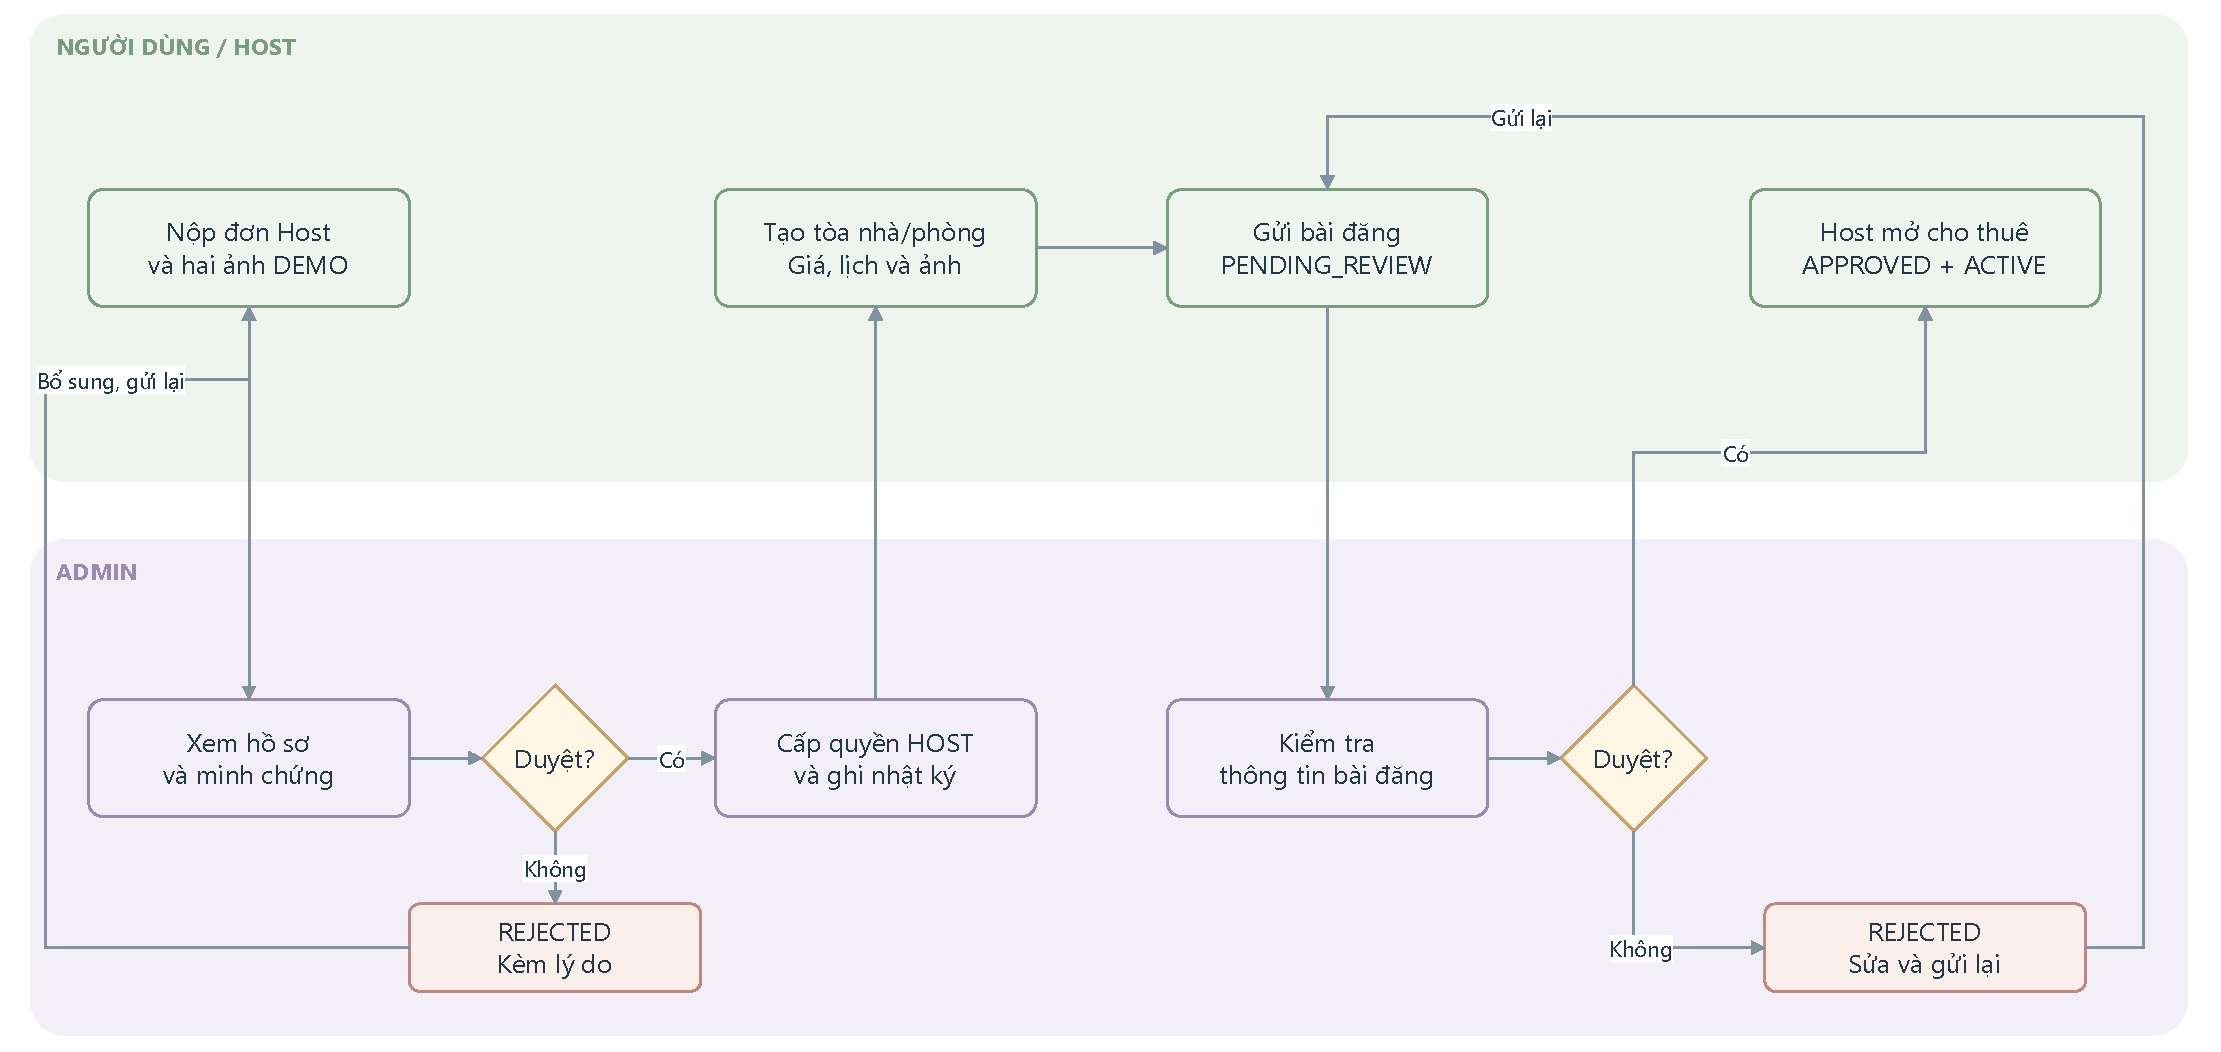
\includegraphics[page=1,width=\linewidth,height=0.82\textheight,keepaspectratio]{chapter2/workflow_diagram_v2.pdf}
\caption{Quy trình cấp quyền Host và công bố không gian.}\label{fig:app-host-workflow}
\end{figure}
\clearpage\BroomLandscapePagefalse\end{landscape}\pagestyle{fancy}
\clearpage
\begin{landscape}\pagestyle{empty}\BroomLandscapePagetrue
\begin{figure}[p]\centering
\includegraphics[page=2,width=\linewidth,height=0.82\textheight,keepaspectratio]{chapter2/workflow_diagram_v2.pdf}
\caption{Quy trình tạo, giữ lịch và xử lý yêu cầu đặt chỗ.}\label{fig:ch2-booking-workflow}
\end{figure}
\clearpage\BroomLandscapePagefalse\end{landscape}\pagestyle{fancy}
\clearpage
\begin{landscape}\pagestyle{empty}\BroomLandscapePagetrue
\begin{figure}[p]\centering
\includegraphics[page=3,width=\linewidth,height=0.82\textheight,keepaspectratio]{chapter2/workflow_diagram_v2.pdf}
\caption{Quy trình sử dụng phòng, khép lượt thuê và xác minh ngoại lệ.}\label{fig:app-usage-workflow}
\end{figure}
\clearpage\BroomLandscapePagefalse\end{landscape}\pagestyle{fancy}
\clearpage
\begin{landscape}\pagestyle{empty}\BroomLandscapePagetrue
\begin{figure}[p]\centering
\includegraphics[page=4,width=\linewidth,height=0.82\textheight,keepaspectratio]{chapter2/workflow_diagram_v2.pdf}
\caption{Luồng tạo QR và cập nhật kết quả thanh toán payOS.}\label{fig:app-payment-workflow}
\end{figure}
\clearpage\BroomLandscapePagefalse\end{landscape}\pagestyle{fancy}

\subsection{Sơ đồ phân rã chức năng}
Các chức năng được phân rã từ mục tiêu của từng vai trò đến nhóm thao tác liên quan. Nhóm người thuê bao gồm tài khoản, khám phá, booking, tương tác và hồ sơ Host; nhóm Host tập trung vào phòng, lịch và vận hành lượt thuê; nhóm Admin tập trung vào xét duyệt, xử lý vi phạm và kiểm tra nghiệp vụ. Cách phân rã tại Hình~\ref{fig:ch2-functions} làm rõ trách nhiệm mà không đồng nhất mỗi màn hình với một chức năng độc lập.

\begin{figure}[H]\centering
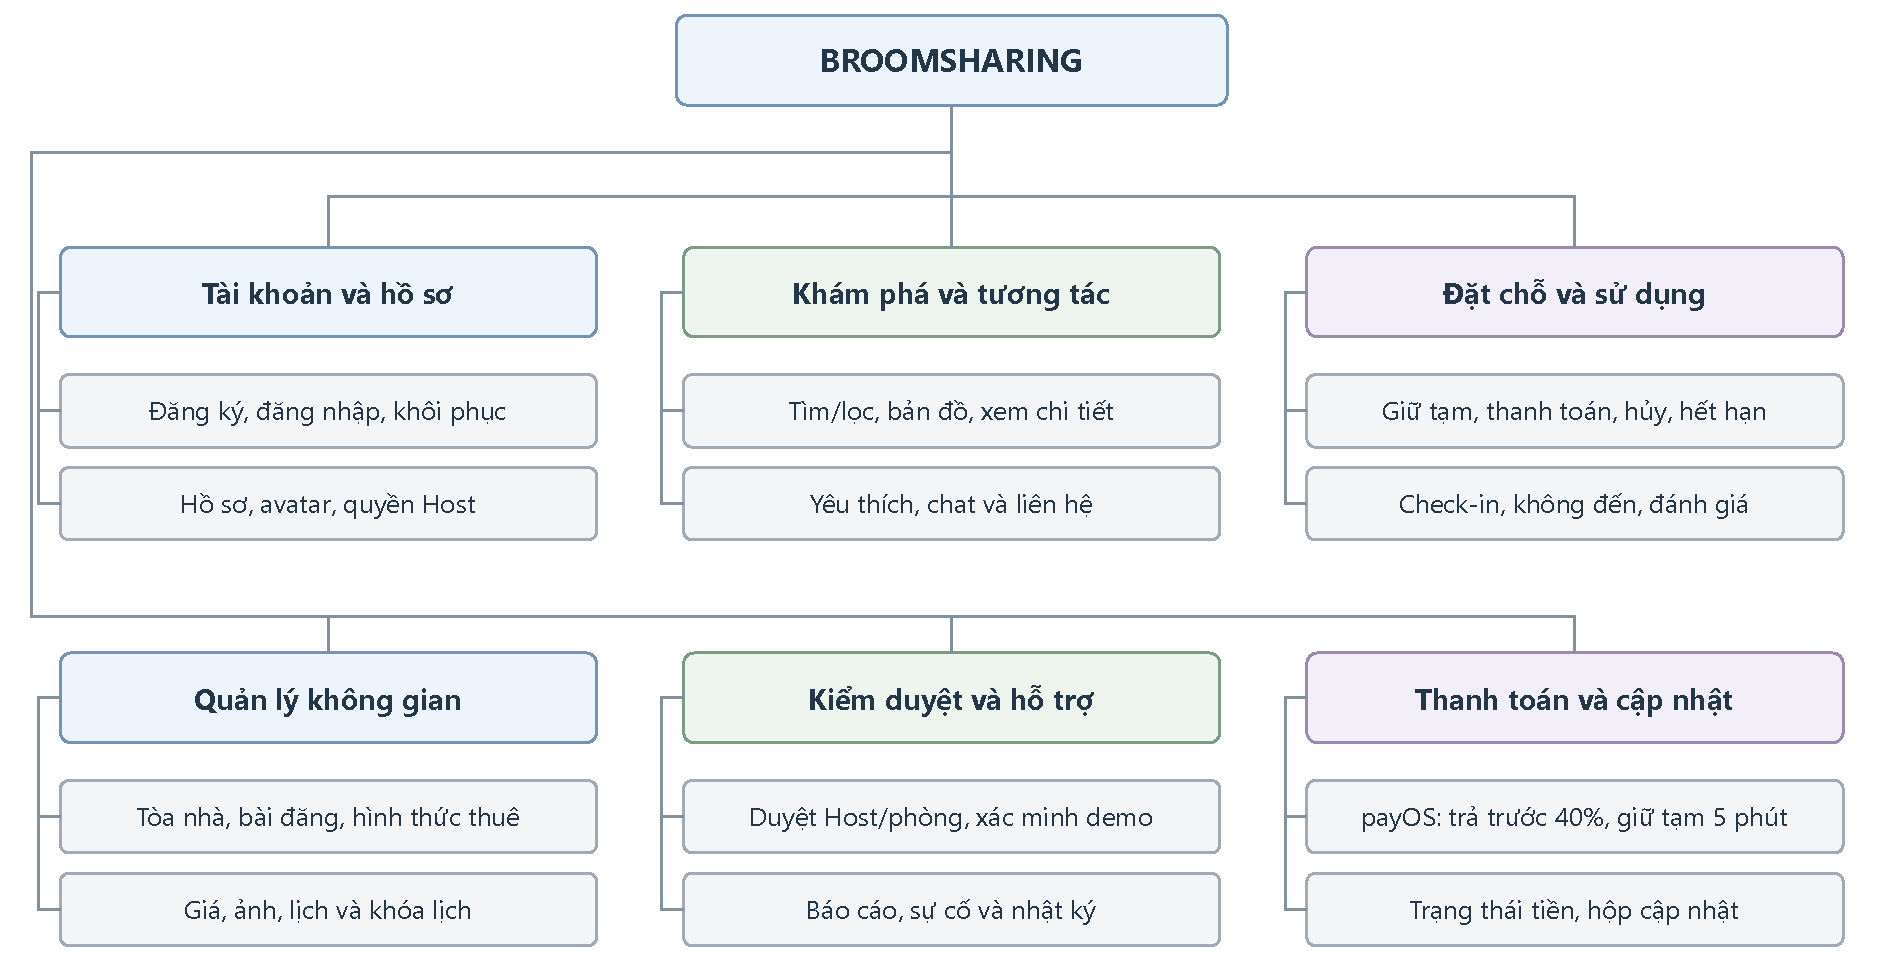
\includegraphics[page=1,width=\textwidth]{chapter2/usecase_decomposition_v2.pdf}
\caption{Phân rã chức năng tổng quát của BroomSharing.}\label{fig:ch2-functions}
\end{figure}

Chức năng tin nhắn hỗ trợ trao đổi giữa hai bên của một hội thoại. Hộp cập nhật tổng hợp sự kiện booking và trạng thái đã đọc của từng tài khoản. Đánh giá gắn với lượt đã sử dụng, còn báo cáo vi phạm được chuyển đến Admin và cho phép Host phản hồi. Các chức năng này bổ sung thông tin xử lý cho lượt thuê, đồng thời duy trì giới hạn truy cập theo vai trò và chủ thể liên quan.

Các nhánh phân rã theo từng nhóm được trình bày tại \hyperref[app:chapter2-details]{Phụ lục G}.

\subsection{Sơ đồ use case}
Hình~\ref{fig:ch2-usecase-overview} mô tả các mục tiêu tương tác với hệ thống. Host kế thừa khả năng thuê phòng của người thuê và có thêm nhóm chức năng cho thuê. Admin có tuyến chức năng kiểm duyệt riêng; quyền quản trị không mặc định bao gồm đọc hội thoại riêng của người dùng.

\begin{figure}[H]\centering
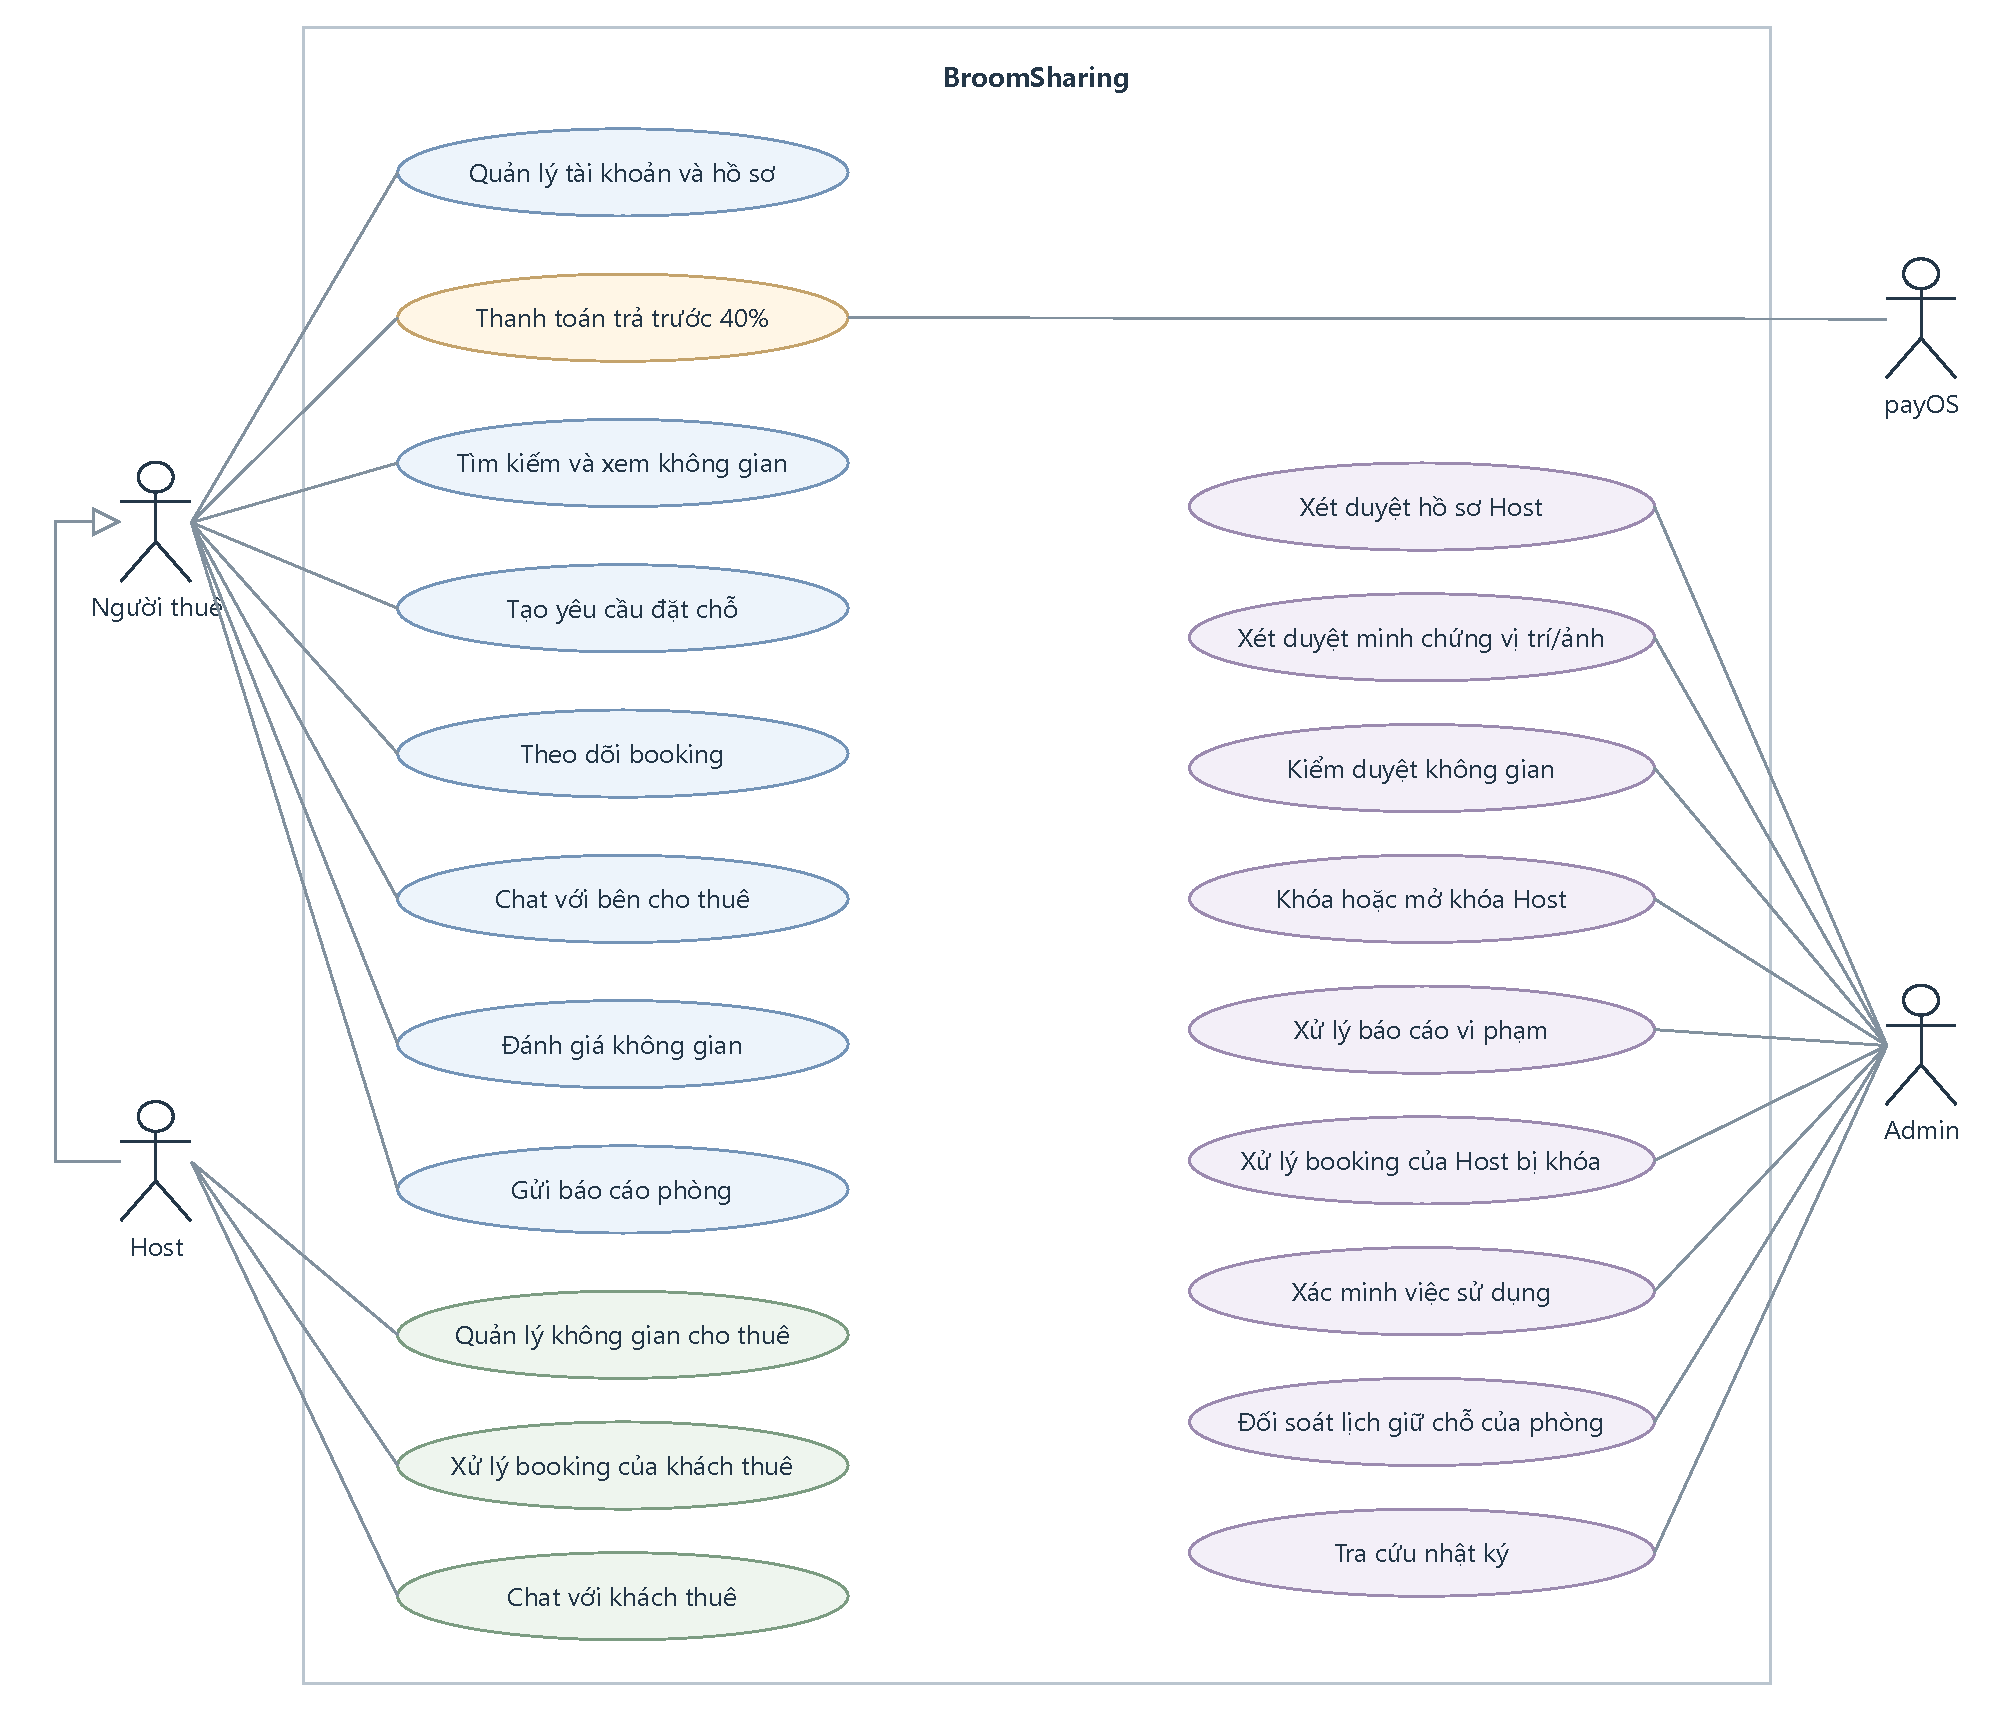
\includegraphics[page=1,width=0.95\textwidth]{chapter2/usecase_diagram_v2.pdf}
\caption{Use case tổng quát với các tác nhân người thuê, Host, Admin và dịch vụ thanh toán.}\label{fig:ch2-usecase-overview}
\end{figure}

Ở phân hệ người thuê, đặt chỗ luôn bao gồm kiểm tra khả dụng và mở bước thanh toán, còn hủy booking là thao tác có điều kiện trên lượt đang được theo dõi. Gửi đơn làm Host bao gồm cung cấp hai ảnh DEMO. Các phân hệ Host và Admin giữ liên kết tác nhân với mục tiêu nghiệp vụ; những cập nhật lịch và nhật ký được mô tả trong quy trình xử lý. Hình~\ref{fig:app-usecase-guest}, Hình~\ref{fig:app-usecase-host} và Hình~\ref{fig:app-usecase-admin} trình bày chi tiết mục tiêu của từng phân hệ.


\clearpage
Phân hệ người thuê bao quát truy cập tài khoản, khám phá, đặt chỗ và tương tác sau thuê. Kiểm tra khả dụng và mở thanh toán thuộc thao tác đặt chỗ; hủy booking chỉ thực hiện khi lượt thuê còn đáp ứng điều kiện hủy.
\begin{figure}[H]\centering
\includegraphics[page=2,width=\textwidth,height=0.75\textheight,keepaspectratio]{chapter2/usecase_diagram_v2.pdf}
\caption{Use case chi tiết của người thuê.}\label{fig:app-usecase-guest}
\end{figure}
\clearpage
Host quản lý tòa nhà, phòng, giá và lịch, đồng thời ghi nhận việc sử dụng và các ngoại lệ của lượt thuê. Quyền thuê dùng chung được kế thừa tại sơ đồ tổng quát; trang này tập trung vào các mục tiêu cho thuê.
\begin{figure}[H]\centering
\includegraphics[page=3,width=\textwidth,height=0.80\textheight,keepaspectratio]{chapter2/usecase_diagram_v2.pdf}
\caption{Use case chi tiết của Host.}\label{fig:app-usecase-host}
\end{figure}
\clearpage
Admin xét duyệt hồ sơ, bài đăng và minh chứng, xử lý vi phạm và can thiệp các booking thuộc phạm vi quản trị. Xác minh việc sử dụng và đối soát lịch được tách thành các mục tiêu riêng để phản ánh điều kiện xử lý khác nhau.
\begin{figure}[H]\centering
\includegraphics[page=4,width=\textwidth,height=0.80\textheight,keepaspectratio]{chapter2/usecase_diagram_v2.pdf}
\caption{Use case chi tiết của Admin.}\label{fig:app-usecase-admin}
\end{figure}

\subsection{Đặc tả các nghiệp vụ tiêu biểu}
\subsubsection{Gửi yêu cầu đặt chỗ}
Mục tiêu của nghiệp vụ là tạo lượt thuê có giá và quyền giữ lịch xác định. Điều kiện đầu vào gồm tài khoản được phép thuê, phòng đã duyệt và hoạt động, Host hợp lệ và thời gian chưa bắt đầu; không được đặt phòng của chính mình. Với thuê theo giờ, khoảng chọn phải đáp ứng ngày làm việc, giờ mở cửa và thời lượng tối thiểu. Cả hai chế độ đều được kiểm tra khoảng khóa liên quan.

Với thuê theo giờ, ứng dụng xác định các slot kỹ thuật 30 phút cần giữ trong khoảng được chọn; với thuê cố định, yêu cầu giữ toàn bộ một hoặc ba tháng. Hai chế độ không được dùng đồng thời cho cùng phòng. Mức giá dự kiến trên giao diện chỉ phục vụ xác nhận lựa chọn; trước khi tạo booking, dữ liệu phòng và lịch tiếp tục được kiểm tra trong transaction. Kết quả thành công là booking \texttt{PENDING} cùng các khóa lịch tương ứng, chưa phải booking đã thanh toán thành công. Màn hình tiếp theo mở QR; backend mới có quyền xác nhận kết quả nhận tiền.

Nhánh không thành công phân biệt dữ liệu nhập không phù hợp với lịch vừa bị người khác giữ. Nếu hai tài khoản gửi yêu cầu trùng nhau, chỉ yêu cầu còn thỏa điều kiện khi ghi dữ liệu được chấp nhận. Khi gửi lại cùng định danh yêu cầu và cùng nội dung, Repository trả về booking đã có thay vì tạo thêm bản ghi. Cách xử lý này tránh tạo lặp khi kết quả phản hồi chậm hoặc người dùng gửi lại thao tác.

\subsubsection{Điều kiện xử lý và khép lượt thuê}
Mỗi thao tác phải kiểm tra trạng thái hiện tại và quyền của người thực hiện, kể cả khi nút xử lý đã được hiển thị trước đó. Đối với hủy thông thường, booking phải còn ở trạng thái cho phép và chưa tới giờ bắt đầu; Host phải cung cấp lý do. Kết quả được lưu cùng người xử lý và mốc thời gian để các bên nhận biết nguồn gốc thay đổi.

Khi khép lượt, hệ thống giải phóng đúng lịch do booking đó giữ và bảo toàn lịch sử. Nếu Admin bổ sung xác nhận sử dụng hoặc sửa kết luận không đến, thao tác chỉ cập nhật kết quả liên quan, không nhả lịch lần thứ hai. Quyền đánh giá được kiểm tra từ người thuê, trạng thái đã khép và xác nhận sử dụng, thay vì chỉ dựa vào việc thời gian thuê đã kết thúc.

\subsubsection{Báo cáo vi phạm và xử lý quản trị}
Người thuê gửi báo cáo đối với phòng, mô tả vấn đề cần giải quyết; Host có thể phản hồi khi báo cáo còn mở. Admin xem thông tin đối tượng cùng phản hồi trước khi giải quyết hoặc bác báo cáo. Nếu cần hạn chế hoạt động, Admin có thể đình chỉ phòng hoặc khóa Host trong phạm vi thao tác được hỗ trợ. Báo cáo là hồ sơ xử lý vi phạm, không thay thế đánh giá của khách về một lượt sử dụng.

Đình chỉ phòng làm thay đổi khả năng nhận yêu cầu mới, nhưng không xóa lịch sử booking. Với Host bị khóa, các lượt chưa khép phải được xem xét từng trường hợp theo quy trình ngoại lệ. Việc gỡ đình chỉ cũng không tự mở phòng trở lại cho thuê: phòng chuyển về không hoạt động để Host chủ động kiểm tra trước khi công bố. Cách tách các quyết định này giúp tránh một thao tác quản trị làm thay đổi ngoài ý muốn toàn bộ vòng đời của các lượt thuê liên quan.

\subsection{Yêu cầu phi chức năng và các ràng buộc thiết kế}
Về tính nhất quán, một phòng chỉ được giữ độc quyền trong khoảng thuê, kể cả trong thời hạn tạm giữ chờ thanh toán. Các thay đổi booking, lịch và thông tin kiểm soát của phòng phải cùng thành công hoặc cùng bị từ chối trong thao tác tương ứng. Lịch không được chỉnh bằng cách chỉ ẩn một booking trên giao diện; các khóa đang giữ phải được giải phóng theo chính bản ghi đã tạo chúng.

Về phân quyền, ứng dụng kiểm tra cả vai trò và quan hệ với đối tượng. Host chỉ quản lý tài sản thuộc sở hữu; người thuê chỉ thực hiện quyền của mình trên booking; thành viên hội thoại mới được đọc và gửi tin trong hội thoại đó. Firestore Security Rules cho phép kiểm tra danh tính và dữ liệu trong điều kiện cho phép hoặc từ chối thao tác \parencite{firebase_rules_conditions}. Backend thanh toán sử dụng thông tin xác thực và kiểm tra nghiệp vụ phía máy chủ, không lấy số tiền do màn hình tự khai báo làm căn cứ thu tiền.

Về khả năng sử dụng, giao diện phân biệt đang tải, danh sách trống, lỗi và kết quả thành công. Khi dữ liệu thay đổi từ tài khoản khác, màn hình cần cập nhật trạng thái và kiểm tra lại trước thao tác quan trọng. Lỗi kết nối phải có phản hồi và cho phép thử lại khi phù hợp, đồng thời tránh tạo lặp dữ liệu. Các yêu cầu này được đánh giá qua kịch bản thao tác trên thiết bị và kết nối cụ thể.
